\documentclass[10pt,a4paper]{article}
\usepackage[utf8]{inputenc}
\usepackage[ngerman]{babel}
\usepackage[left=2.5cm,right=2.5cm,top=4cm,bottom=3cm]{geometry} % Seitenränder 
\usepackage{amsmath}
\usepackage{amsfonts}
\usepackage{amssymb}
\usepackage{graphicx}
\usepackage{mathabx} % contains \Dashv
\usepackage{enumitem}
\usepackage{fancyhdr}
\usepackage{tikz}

\title{Informatik der Syteme - Exercise 4}
\author{Jan Hoffmann; Mike Hengge}
\pagestyle{fancy}
% Header
\fancyhead[L]{\textbf{Informatik der Systeme}\\ \textbf{Exercise 4}}
\fancyhead[C]{}
\fancyhead[R]{Jan Hoffmann, Matr. 3177642\\ Mike Hengge, Matr. 3940400}
% Footer
\fancyfoot[L]{}
\fancyfoot[C]{}
\fancyfoot[R]{\thepage}

\begin{document}
\section*{Problem 4.1:}
\begin{enumerate}
  \item $\frac {m}{n} = f(k)$  \\ 
					Da $ n = 2^k - 1 $\ und$ $ m = 2^k - k - 1$, ist $f(k) = \frac {2^k - k - 1}{2^k - 1}$. \\
					$f(1) = 0$, $f(2) = \frac{1}{3}$,..., $f(12) = \frac{4083}{4095} \\ 
					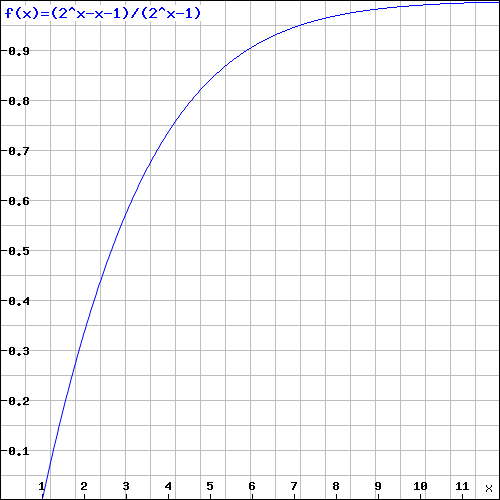
\includegraphics[scale=0.4]{graph.png}
	\setcounter{MaxMatrixCols}{20}$
	\item $2^k-k-1 = 11$ \Rightarrow k = 4 \\\\
				$\begin{pmatrix}
					1 & 0 & 0 & 1 & 0 & 1 & 0 & 1 & 1 & 1 & 1 \\
					1 & 1 & 1 & 0 & 0 & 1 & 0 & 1 & 1 & 1 & 1 \\
					1 & 0 & 0 & 1 & 1 & 0 & 1 & 0 & 1 & 1 & 1 \\
					1 & 0 & 0 & 1 & 0 & 1 & 0 & 1 & 0 & 0 & 0 
					
				\end{pmatrix}					
	\item $CW = 0110$ \Rightarrow \ $Kontrollstellen = (0110) * (01101010110) = 0110  $ \\
	\item $a) $Z=$\begin{pmatrix}
									0 \\
									0 \\
									1 \\
									0 \\
								\end{pmatrix} \
				$b) $Z=$\begin{pmatrix}
									1 \\
									1 \\
									0 \\
									0 \\
								\end{pmatrix} \
				$c) $Z=$\begin{pmatrix}
									1 \\
									1 \\
									1 \\
									0 \\
								\end{pmatrix}
$  
	\item 
\end{enumerate}

\section*{Problem 4.2:}
\begin{enumerate}
	\item Anzahl der Nutzworte ist 2^3=8 \\
	000 \\ 001 \\ 010 \\ 011 \\ 100 \\ 101 \\ 110 \\ 111 \\ $
	\item 
				a(0) = 1 \\
				a(1) = 3 \\
				a(2) = 4 \\
				a(3) = 1 \\ 
	\item Hamming-Distanz $h = min(d(C_i, C_j) = min(d(G_2, G_3) = 3$ \\
	\item $G_2 = 10010$ \rightarrow \ Fehlübertragung: \  $10101$ \\
	\Rightarrow \ scheinbar \ fehlerloses \ G3, \ ist \ aber \ fehlerhaftes \ G2. \\
	\item $G*_1 = 011$ \ \ $G*_2 = 100$ \ \ $G*_3 = 101$
												
	
\end{enumerate}

\section*{Problem 4.3:}
\begin{enumerate}
	\item$p$ ist Bitfehlerwahrscheinlichkeit\\
		Wahrscheinlichkeit, dass ein Bit korrekt übertragen wird ist $1-p$\\
		Wahrscheinlichkeit für $m$ korrekt übertragene Bits ist $(1-p)^m$
	\item
		\begin{align*}
			\text{Anzahl übertragener Bits} &= m\\
			P(\text{Bitfehler}) &= p\\
			P(\text{Bit korrekt}) &= (1-p)\\
			P(n \text{ von } m \text{ Bits fehlerhaft}) &= (1 - p)^{m-n} \cdot p^n \cdot \underbrace{\frac{m!}{(m-n)!n!}}_{Permutationen} \\
			P(1\text{ von } m \text{ Bit fehlerhaft}) &= (1-p)^{m-1} \cdot p \cdot m
		\end{align*}
	\item
		Sei $CW_h$ ein Codewort aus einem Hamming-Code mit der Hamming-Distanz $h$\\		
		\begin{align*}	
			n &= \text{ Länge von }CW_h \\
			\eta &= \left\lfloor \frac{h-1}{2} \right\rfloor \text{ ist die Anzahl der korrigierbaren Fehler.} \\
			P(\text{höchstens } \eta \text{ von } n \text{ Bit fehlerhaft}) 
				&= \sum_{i=0}^{\eta}{(1 - p)^{n-i} \cdot p^i} \cdot \frac{n!}{(n-i)!i!}\\
		\end{align*}
		Die Wahrscheinlichkeit ein Code-Wort korrekt (oder korrigierbar) zu übertragen wird also größer, je mehr Fehler Korrigierbar sind.	
\end{enumerate}

\end{document}